\begin{flushleft}
Abbiamo implementato il codice seguente per poter rispondere alle domande dell'esercizio:
\lstinputlisting[language=Matlab]{cap_3/es16/es16.m}
Possiamo confermare che le soluzioni $x$ e $y$ dei sistemi lineari $A\cdot x = b$ e $A\cdot y = c$ sono giuste dato che calcolando i loro residui otteniamo:
\begin{figure}[h]
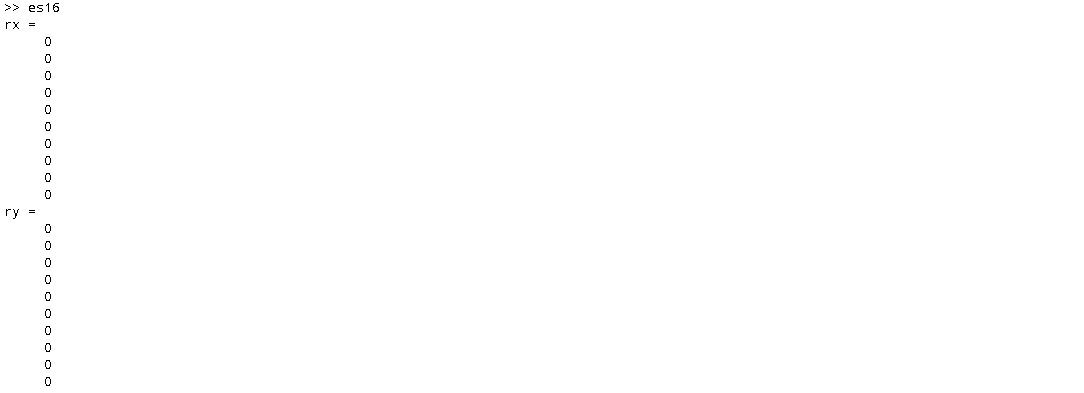
\includegraphics[left, width=250px]{cap_3/es16/es316}
\end{figure}
\newline \\
Nel passo successivo si usa la serie di istruzioni forniteci dall'esercizio. Nel caso del vettore $x$ si perviene alla stessa soluzione precedentemente fornita dall'esercizio. Invece nel caso del vettore $y$ abbiamo una propagazione degli errori nella soluzione trovata, che si può vedere a partire dall'elemento $y_7$. Possiamo vederlo dall'output:
\begin{figure}[h]
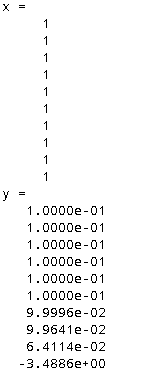
\includegraphics[left, width=250px]{cap_3/es16/es316a}
\end{figure}
\newline \\
Si vede che c'è una perturbazione sulla soluzione che è possibile spiegare andando a studiare la seguente disuguaglianza:
\[
\frac{\left|\left|\Delta x\right|\right|}{\left|\left|x\right|\right|} \leq k(A) \cdot \left(\frac{\left|\left|\Delta c\right|\right|}{\left|\left|c\right|\right|} + \frac{\left|\left|\Delta A\right|\right|}{\left|\left|A\right|\right|}\right) = k(A) \cdot \left(\frac{\left|\left|\Delta c\right|\right|}{\left|\left|0.1\cdot b\right|\right|} + \frac{\left|\left|\Delta A\right|\right|}{\left|\left|A\right|\right|}\right) = 
\]
\[
= k(A) \cdot \left(\frac{\left|\left|\Delta c\right|\right|}{10^{-1}\cdot\left|\left|b\right|\right|} + \frac{\left|\left|\Delta A\right|\right|}{\left|\left|A\right|\right|}\right) = k(A) \cdot \left(10\cdot\frac{\left|\left|\Delta c\right|\right|}{\left|\left|b\right|\right|} + \frac{\left|\left|\Delta A\right|\right|}{\left|\left|A\right|\right|}\right) 
\]
Considerato che:
\begin{itemize}
    \item $\frac{\left|\left|\Delta x\right|\right|}{\left|\left|x\right|\right|}$ può essere assimilato ad una sorta di errore relativo sul risultato
    \item $\frac{\left|\left|\Delta A\right|\right|}{\left|\left|A\right|\right|}$ e $\frac{\left|\left|\Delta c\right|\right|}{\left|\left|c\right|\right|}$ possono essere assimilati ai corrispondenti errori relativi sui dati in ingresso
\end{itemize}
dato che il numero di condizionamento del problema è $k(A)=1.0202\cdot10^{20}$, che è $>>1$ (calcolato nell'esercizio precedente a pag. \pageref{es315}), allora la matrice è mal condizionata.
\end{flushleft}